\chapter{Array-Based Lists}
\chaplabel{arrays}

In this chapter, we study implementations of the #List# and #Queue#
interfaces where the underlying data is stored in an array, called the
\emph{backing array}.  The following table summarizes the running times
of operations for the data structures presented in this chapter:

\begin{center}
\begin{tabular}{|l|l|l|} \hline
 & #get(i)#/#set(i,x)# & #add(i,x)#/#remove(i)# \\ \hline
#ArrayStack# & $O(1)$ & $O(#n#-#i#)$ \\
#ArrayDeque# & $O(1)$ & $O(\min\{#i#,#n#-#i#\})$ \\
#DualArrayDeque# & $O(1)$ & $O(\min\{#i#,#n#-#i#\})$ \\
#RootishArrayStack# & $O(1)$ & $O(#n#-#i#)$ \\ \hline
\end{tabular}
\end{center}

Data structures that work by storing data in a single array have many
advantages and limitations in common:
\begin{itemize}
  \item Arrays offer constant time access to any value in the array.
  This is what allows #get(i)# and #set(i,x)# to run in constant time.

  \item Arrays are not very dynamic.  Adding or removing an element
  near the middle of a list means that a large number of elements in the
  array need to be shifted to make room for the newly added element or
  to fill in the gap created by the deleted element.  This is why the
  operations #add(i,x)# and #remove(i)# have running times that depend
  on #n# and #i#.

  \item Arrays cannot expand or shrink.  When the number of elements in
  the data structure exceeds the size of the backing array, a new array needs
  to be allocated and the data from the old array needs to be copied
  into the new array.  This is an expensive operation.
\end{itemize}
The third point is important.  The running times cited in the table
above do not include the cost of growing and shrinking the backing array.
We will see that, if carefully managed, the cost of growing and shrinking
the backing array does not add much to the cost of an \emph{average}
operation.  More precisely, if we start with an empty data structure,
and perform any sequence of $m$ #add(i,x)# or #remove(i)# operations,
then the total cost of growing and shrinking the backing array, over the
entire sequence of $m$ operations is $O(m)$.  Although some individual
operations are more expensive, the amortized cost, when amortized over
all $m$ operations, is only $O(1)$ per operation.

\cpponly{
In this chapter, and throughout this book, it will be convenient to
have arrays that keep track of their size.  The usual C++ arrays do
not do this, so we have defined a class,  #array#, that keeps track
of its length.  The implementation of this class is straightforward.
It is implemented as a standard C++ array, #a#, and an integer, #length#:}
\cppimport{ods/array.a.length}
\cpponly{
The size of an #array# is specified at the time of creation:
}
\cppimport{ods/array.array(len)}
\cpponly{The elements of an array can be indexed:}
\cppimport{ods/array.operator[]}
\cpponly{Finally, when one array is assigned to another, this is just
a pointer manipulation that takes constant time:}
\cppimport{ods/array.operator=}

\section{#ArrayStack#: Fast Stack Operations Using an Array}
\seclabel{arraystack}

An #ArrayStack# implements the list interface using an array #a#, called
the \emph{backing array}.  The list element with index #i# is stored
in #a[i]#.  At most times, #a# is larger than strictly necessary,
so an integer #n# is used to keep track of the number of elements
actually stored in #a#.  In this way, the list elements are stored in
#a[0]#,\ldots,#a[n-1]# and, at all times, $#a.length# \ge #n#$.

\codeimport{ods/ArrayStack.a.n.size()}

\subsection{The Basics}

Accessing and modifying the elements of an #ArrayStack# using #get(i)#
and #set(i,x)# is trivial. After performing any necessary bounds-checking
we simply return or set, respectively, #a[i]#.

\codeimport{ods/ArrayStack.get(i).set(i,x)}

The operations of adding and removing elements from an #ArrayStack#
are illustrated in \figref{arraystack}.  To implement the #add(i,x)#
operation, we first check if #a# is already full.  If so, we call
the method #resize()# to increase the size of #a#.  How #resize()#
is implemented will be discussed later.  For now, it is sufficient to
know that, after a call to #resize()#, we can be sure that $#a.length#
> #n#$.  With this out of the way, we now shift the elements
$#a[i]#,\ldots,#a[n-1]#$ right by one position to make room for #x#,
set #a[i]# equal to #x#, and increment #n#.

\begin{figure}
  \begin{center}
    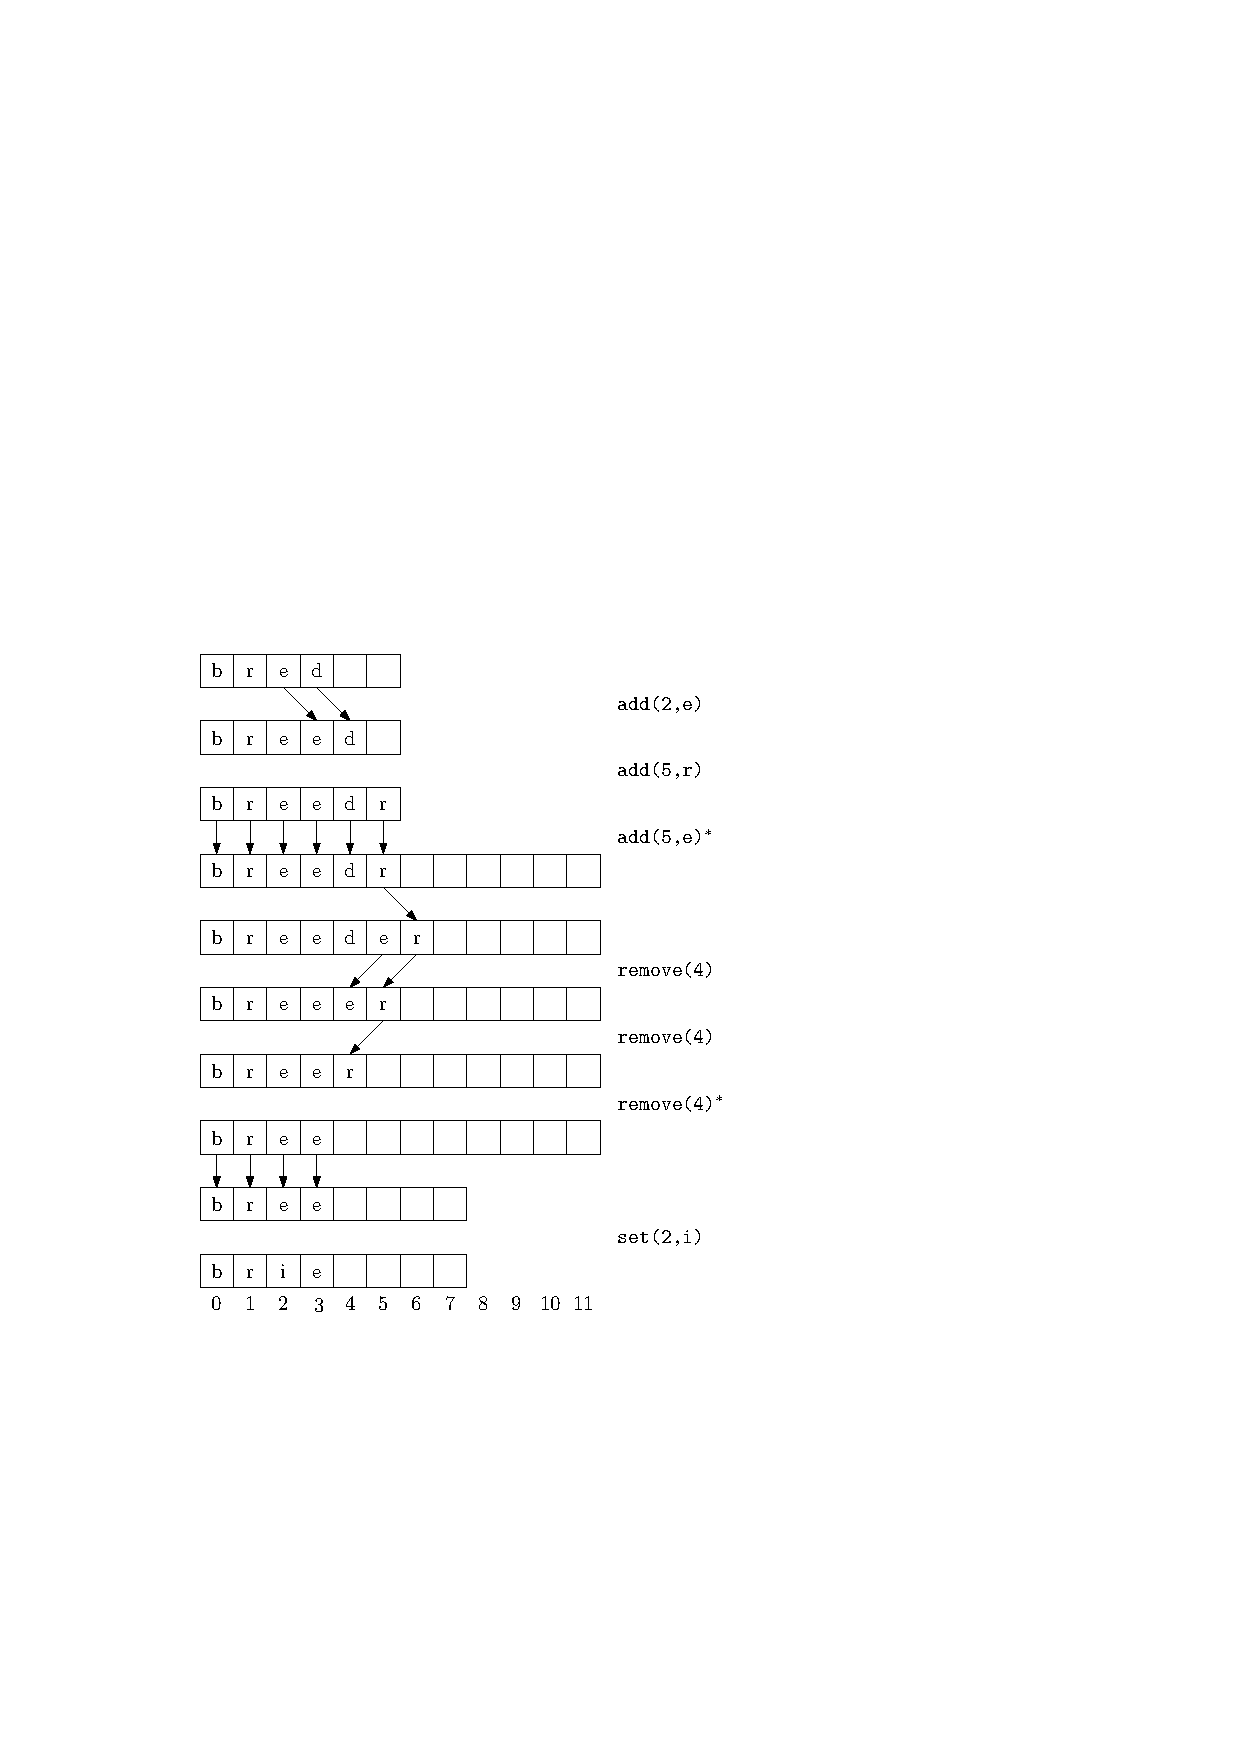
\includegraphics{figs/arraystack}
  \end{center}
  \caption[Adding to an ArrayStack]{A sequence of #add(i,x)# and #remove(i)# operations on an
  #ArrayStack#.  Arrows denote elements being copied.  Operations that
  result in a call to #resize()# are marked with an asterisk.}
  \figlabel{arraystack}
\end{figure}

\codeimport{ods/ArrayStack.add(i,x)}
% TODO: Add shifting figure
If we ignore the cost of the potential call to #resize()#, the cost of the
#add(i,x)# operation is proportional to the number of elements we have
to shift to make room for #x#.  Therefore the cost of this operation
(ignoring the cost of resizing #a#) is $O(#n#-#i#+1)$.

Implementing the #remove(i)# operation is similar.  We shift the elements
$#a[i+1]#,\ldots,#a[n-1]#$ left by one position (overwriting #a[i]#) and
decrease the value of #n#.  After doing this, we check if #n# is getting
much smaller than #a.length# by checking if $#a.length# \ge 3#n#$. If so,
we call #resize()# to reduce the size of #a#.

\codeimport{ods/ArrayStack.remove(i)}
% TODO: Add shifting figure
If we ignore the cost of the #resize()# method, the cost of a #remove(i)#
operation is proportional to the number of elements we shift, which
is $O(#n#-#i#)$.

\subsection{Growing and Shrinking}

The #resize()# method is fairly straightforward; it allocates a new
array #b# whose size is $2#n#$ and copies the #n# elements of #a# into
the first #n# positions in #b#, and then sets #a# to #b#. Thus, after a call to #resize()#, $#a.length# = 2#n#$.

\codeimport{ods/ArrayStack.resize()}

Analyzing the actual cost of the #resize()# operation is easy. It
allocates an array #b# of size $2#n#$ and copies the #n# elements of #a#
into #b#.  This takes $O(#n#)$ time.

The running time analysis from the previous section ignored the cost
of calls to #resize()#.  In this section we analyze this cost using a
technique known as \emph{amortized analysis}.  This technique does not
try to determine the cost of resizing during each individual #add(i,x)#
and #remove(i)# operation.  Instead, it considers the cost of all calls to
#resize()# during a sequence of $m$ calls to #add(i,x)# or #remove(i)#.
In particular, we will show:

\begin{lem}\lemlabel{arraystack-amortized}
  If an empty #ArrayList# is created and any sequence of $m\ge 1$ calls
  to #add(i,x)# and #remove(i)# are performed, then the total time spent
  during all calls to #resize()# is $O(m)$.
\end{lem}

\begin{proof}
  We will show that anytime #resize()# is called, the number of calls
  to #add# or #remove# since the last call to #resize()# is at least
  $#n#/2-1$.  Therefore, if $#n#_i$ denotes the value of #n# during the
  $i$th call to #resize()# and $r$ denotes the number of calls to
  #resize()#, then the total number of calls to #add(i,x)# or
  #remove(i)# is at least
  \[
     \sum_{i=1}^{r} (#n#_i/2-1) \le m  \enspace ,
  \]
  which is equivalent to
  \[
    \sum_{i=1}^{r} #n#_i \le 2m + 2r  \enspace .
  \]
  On the other hand, the total time spent during all calls to #resize()# is 
  \[
     \sum_{i=1}^{r} O(#n#_i) \le O(m+r) = O(m)  \enspace ,
  \]
  which will prove the lemma since $r$ is not more than $m$.  All
  that remains is to show that the number of calls to #add(i,x)# or
  #remove(i)# between the $(i-1)$th and the $i$th call to #resize()#
  is at least $#n#_i/2$.

  There are two cases to consider. In the first case, #resize()# is
  being called by #add(i,x)# because the backing array #a# is full, i.e.,
  $#a.length# = #n#=#n#_i$.  Consider the previous call to #resize()#:
  After this previous call, the size of #a# was #a.length#, but the
  number of elements stored in #a# was at most $#a.length#/2=#n#_i/2$.
  But now the number of elements stored in #a# is $#n#_i=#a.length#$,
  so there must have been at least $#n#_i/2$ calls to #add(i,x)# since
  the previous call to #resize()#.
  % TODO: Add figure
  
  The second case to consider is when #resize()# is being called by
  #remove(i)# because $#a.length# \ge 3#n#=3#n#_i$.  Again, after the
  previous call to #resize()# the number of elements stored in #a# was
  at least $#a.length/2#-1$.\footnote{The ${}-1$ in this formula accounts for
  the special case that occurs when $#n#=0$ and $#a.length# = 1$.} Now there
  are $#n#_i\le#a.length#/3$ elements stored in #a#.  Therefore, the number
  of #remove(i)# operations since the last call to #resize()# is at least
  \[
      #a.length#/2 - 1 - #a.length#/3 = #a.length#/6 - 1
         = (#a.length#/3)/2 - 1\ge #n#_i/2 -1\enspace .
  \]
  In either case, the number of calls to #add(i,x)# or #remove(i)# that
  occur between the $(i-1)$th call to #resize()# and the $i$th call to
  #resize()# is at least $#n#_i/2-1$, as required to complete the proof.
\end{proof}

\subsection{Summary}

The following theorem summarizes the performance of an #ArrayStack#:

\begin{thm}\thmlabel{arraystack}
  An #ArrayStack# implements the #List# interface.  Ignoring the cost of
  calls to #resize()#, an #ArrayStack# supports the operations
  \begin{itemize}
    \item #get(i)# and #set(i,x)# in $O(1)$ time per operation; and
    \item #add(i,x)# and #remove(i)# in $O(1+#n#-#i#)$ time per operation.
  \end{itemize}
  Furthermore, beginning with an empty #ArrayStack#, any sequence of $m$
  #add(i,x)# and #remove(i)# operations results in a total of $O(m)$
  time spent during all calls to #resize()#.
\end{thm}

The #ArrayStack# is an efficient way to implement a #Stack#.
In particular, we can implement #push(x)# as #add(n,x)# and #pop()#
as #remove(n-1)#, in which case these operations will run in $O(1)$
amortized time.

\section{#FastArrayStack#: An Optimized ArrayStack}
\seclabel{fastarraystack}
Much of the work done by an #ArrayStack# involves shifting (by
#add(i,x)# and #remove(i)#) and copying (by #resize()#) of data.
In the implementations shown above, this was done using #for# loops. It
turns out that many programming environments have specific functions
that are very efficient at copying and moving blocks of data.  In C
there are the #memcpy(d,s,n)# and #memmove(d,s,n)# functions. In C++
there is the #std::copy(a0,a1,b)# algorithm.  In Java there is the
#System.arraycopy(s,i,d,j,n)# method.

\codeimport{ods/FastArrayStack.add(i,x).remove(i).resize()}

These functions are usually highly optimized and may even use special
machine instructions that can do this copying much faster than we could do
using a #for# loop.  Although using these functions does not asymptotically
decrease the running times, it can still be a worthwhile optimization.
In the \javaonly{Java}\cpponly{C++} implementations here, the use of \javaonly{#System.arraycopy(s,i,d,j,n)#}\cpponly{#std::copy(a0,a1,b)#}
resulted in speedups of a factor of 2-3 depending on the types of
operations performed.  Your mileage may vary.

\section{#ArrayQueue#: An Array-Based Queue}
\seclabel{arrayqueue}

In this section, we present the #ArrayQueue# data structure, which
implements a FIFO (first-in-first-out) queue; elements are removed (using
the #remove()# operation) from the queue in the same order they are added
(using the #add(x)# operation).

Notice that an #ArrayStack# is a poor choice for an implementation of a
FIFO queue.  The reason is that we must choose one end of the list to
add to and then remove from the other end.  One of the two operations
must work on the head of the list, which involves calling #add(i,x)#
or #remove(i)# with a value of $#i#=0$.  This gives a running time
of $\Theta(n)$.

To obtain an efficient array-based implementation of a queue, we
first notice that the problem would be easy if we had an infinite
array #a#.  We could maintain one index #j# that keeps track of the
next element to remove and an integer #n# that counts the number of
elements in the queue.  The queue elements would always be stored in
\[ #a[j]#,#a[j+1]#,\ldots,#a[j+n-1]# \enspace . \]
Initially, both #j# and #n# would be 
set to 0.  To add an element, we would place it in #a[j+n]# and increment #n#.
To remove an element, we would remove it from #a[j]#, increment #j#, and
decrement #n#.

Of course, the problem with this solution is that it requires an infinite
array.  An #ArrayQueue# simulates this by using a finite array #a#
and \emph{modular arithmetic}.  This is the kind of arithmetic used when
we are talking about the time of day.  For example 10 o'clock plus 5
hours gives 3 o'clock.  Formally, we say that
\[
    10 + 5 = 15 \equiv 3 \pmod{12} \enspace .
\]
We read the latter part of this equation as ``15 is congruent to 3 modulo
12.'' We can also treat $\bmod$ as a binary operator, so that
\[
   15 \bmod 12 = 3 \enspace .
\]

More generally, for an integer $a$ and positive integer $m$, $a \bmod m$
is the unique integer $r\in\{0,\ldots,m-1\}$ such that $a = r + km$ for
some integer $k$.  Less formally, the value $r$ is the remainder we get
when we divide $a$ by $m$.  In many programming languages, including
\javaonly{Java}\cpponly{C++}, the $\bmod$ operator is represented
using the #%# symbol.\footnote{This is sometimes referred to as the
\emph{brain-dead} mod operator since it does not correctly implement
the mathematical mod operator when the first argument is negative.}

Modular arithmetic is useful for simulating an infinite array,
since $#i#\bmod #a.length#$ always gives a value in the range
$0,\ldots,#a.length-1#$.  Using modular arithmetic we can store the
queue elements at array locations
\[ #a[j%a.length]#,#a[(j+1)%a.length]#,\ldots,#a[(j+n-1)%a.length]#
\enspace. \]
This treats #a# like a \emph{circular array} in which array indices
exceeding $#a.length#-1$ ``wrap around'' to the beginning of
the array.
% TODO: figure

The only remaining thing to worry about is taking care that the number
of elements in the #ArrayQueue# does not exceed the size of #a#.

\codeimport{ods/ArrayQueue.a.j.n}

A sequence of #add(x)# and #remove()# operations on an #ArrayQueue# is
illustrated in \figref{arrayqueue}.  To implement #add(x)#, we first
check if #a# is full and, if necessary, call #resize()# to increase
the size of #a#.  Next, we store #x# in
#a[(j+n)%a.length]# and increment #n#.

\begin{figure}
  \begin{center}
    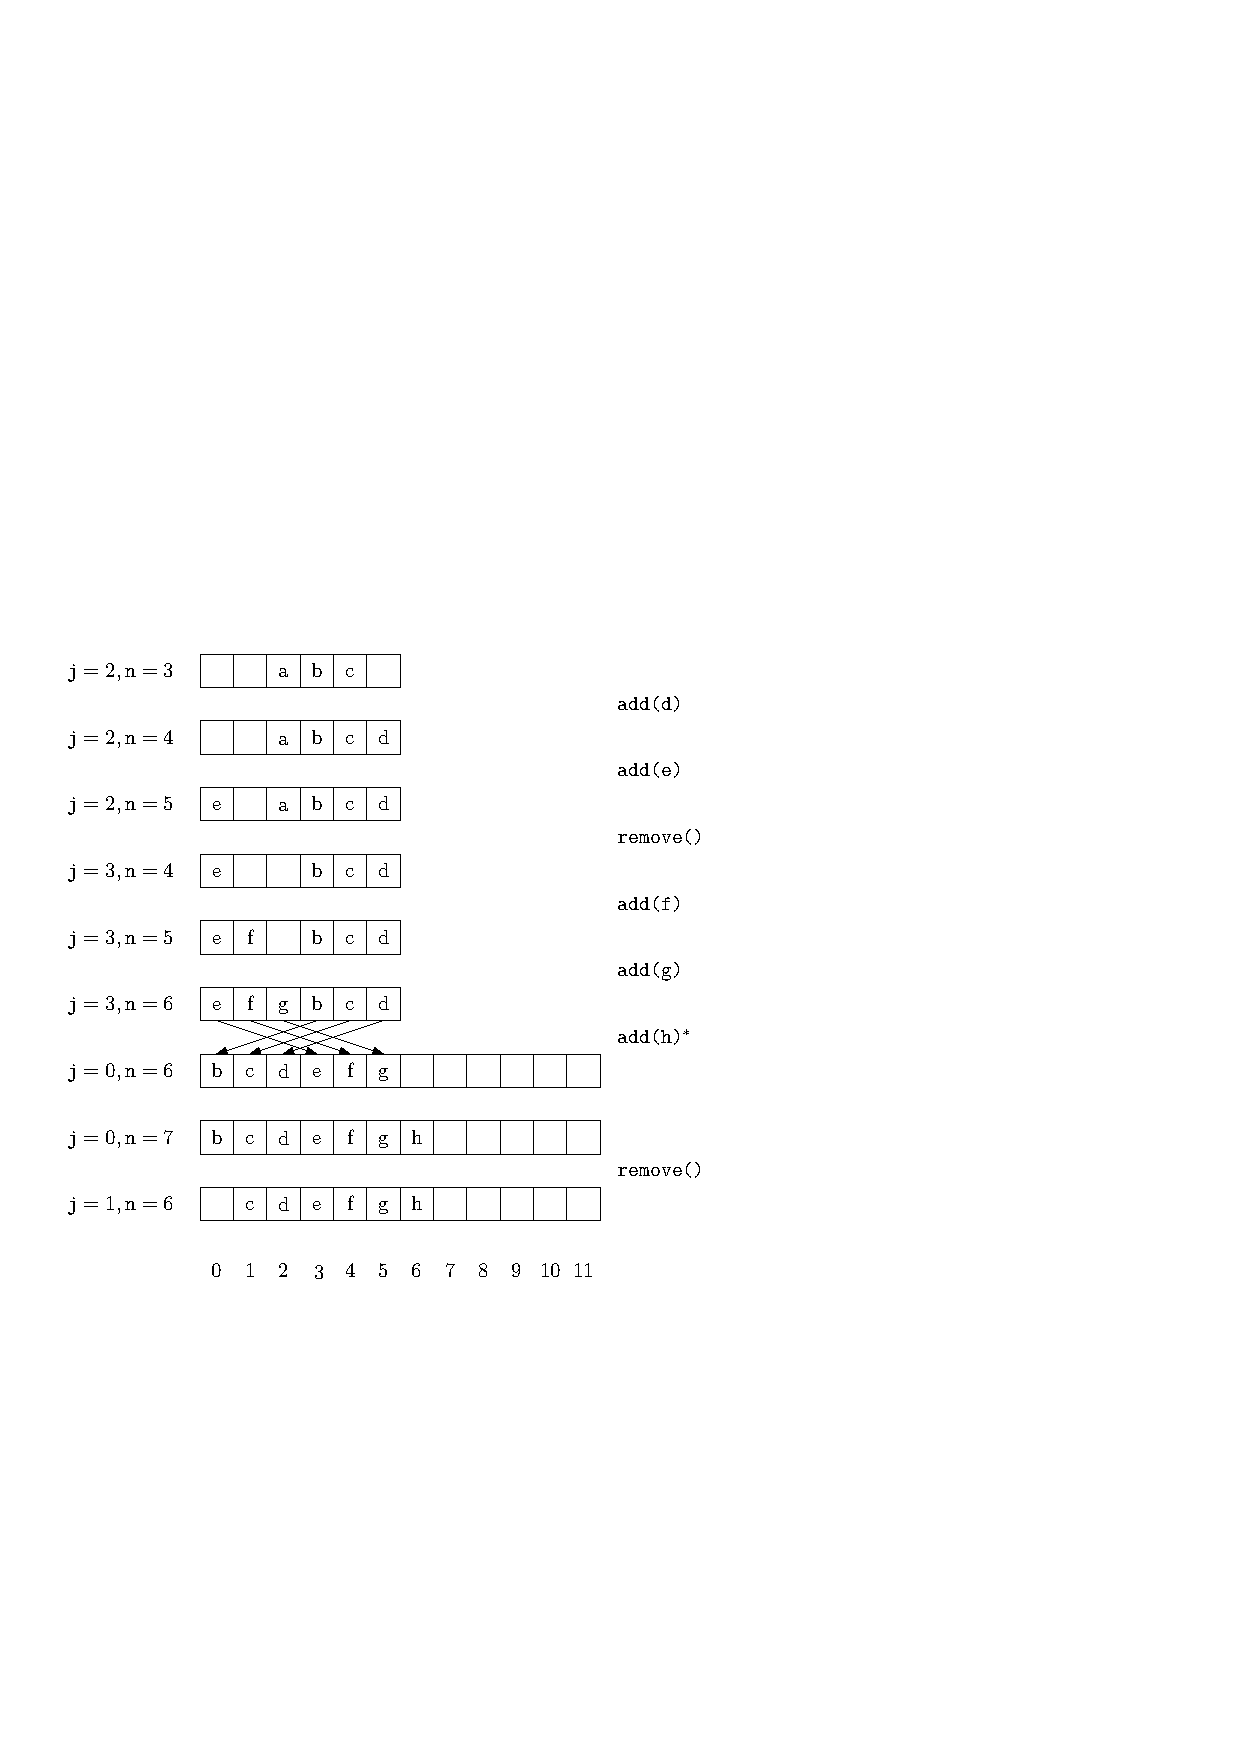
\includegraphics{figs/arrayqueue}
  \end{center}
  \caption[Adding and removing from an ArrayQueue]{A sequence of #add(x)# and #remove(i)# operations on an
  #ArrayQueue#.  Arrows denote elements being copied.  Operations that
  result in a call to #resize()# are marked with an asterisk.}
  \figlabel{arrayqueue}
\end{figure}



\codeimport{ods/ArrayQueue.add(x)}

To implement #remove()# we first store #a[j]# so that we can return
it later.  Next, we decrement #n# and increment #j# (modulo #a.length#)
by setting $#j#=(#j#+1)\bmod #a.length#$.  Finally, we return the stored
value of #a[j]#. If necessary, we may call #resize()# to decrease the
size of #a#.

\codeimport{ods/ArrayQueue.remove()}

Finally, the #resize()# operation is very similar to the #resize()#
operation of #ArrayStack#.  It allocates a new array #b# of size $2#n#$
and copies
\[
   #a[j]#,#a[(j+1)%a.length]#,\ldots,#a[(j+n-1)%a.length]#
\]
onto
\[
   #b[0]#,#b[1]#,\ldots,#b[n-1]#
\]
and sets $#j#=0$.

\codeimport{ods/ArrayQueue.resize()}

\subsection{Summary}

The following theorem summarizes the performance of the #ArrayQueue#
data structure:

\begin{thm}
An #ArrayQueue# implements the (FIFO) #Queue# interface.  Ignoring the cost of
calls to #resize()#, an #ArrayQueue# supports the operations
#add(x)# and #remove()# in $O(1)$ time per operation.
Furthermore, beginning with an empty #ArrayQueue#, any sequence of $m$
#add(i,x)# and #remove(i)# operations results in a total of $O(m)$
time spent during all calls to #resize()#.
\end{thm}

%TODO: Discuss the use of bitwise-and as a replacement for the mod operator

\section{#ArrayDeque#: Fast Deque Operations Using an Array}
\seclabel{arraydeque}

The #ArrayQueue# from the previous section is a data structure
for representing a sequence that allows us to efficiently add to one
end of the sequence and remove from the other end.  The #ArrayDeque#
data structure allows for efficient addition and removal at both ends.
This structure implements the #List# interface using the same circular
array technique used to represent an #ArrayQueue#.

\codeimport{ods/ArrayDeque.a.j.n}

The #get(i)# and #set(i,x)# operations on an #ArrayDeque# are
straightforward.  They get or set the array element $#a[#{#(j+i)#\bmod
#a.length#}#]#$.

\codeimport{ods/ArrayDeque.get(i).set(i,x)}

The implementation of #add(i,x)# is a little more interesting.  As
usual, we first check if #a# is full and, if necessary, call
#resize()# to resize #a#.  Remember that we want this operation to be
fast when #i# is small (close to 0) or when #i# is large (close to
#n#).  Therefore, we check if $#i#<#n#/2$.  If so, we shift the
elements $#a[0]#,\ldots,#a[i-1]#$ left by one position.  Otherwise
($#i#\ge#n#/2$), we shift the elements $#a[i]#,\ldots,#a[n-1]#$ right
by one position.  See \figref{arraydeque} for an illustration of
#add(i,x)# and #remove(x)# operations on an #ArrayDeque#.

\begin{figure}
  \begin{center}
    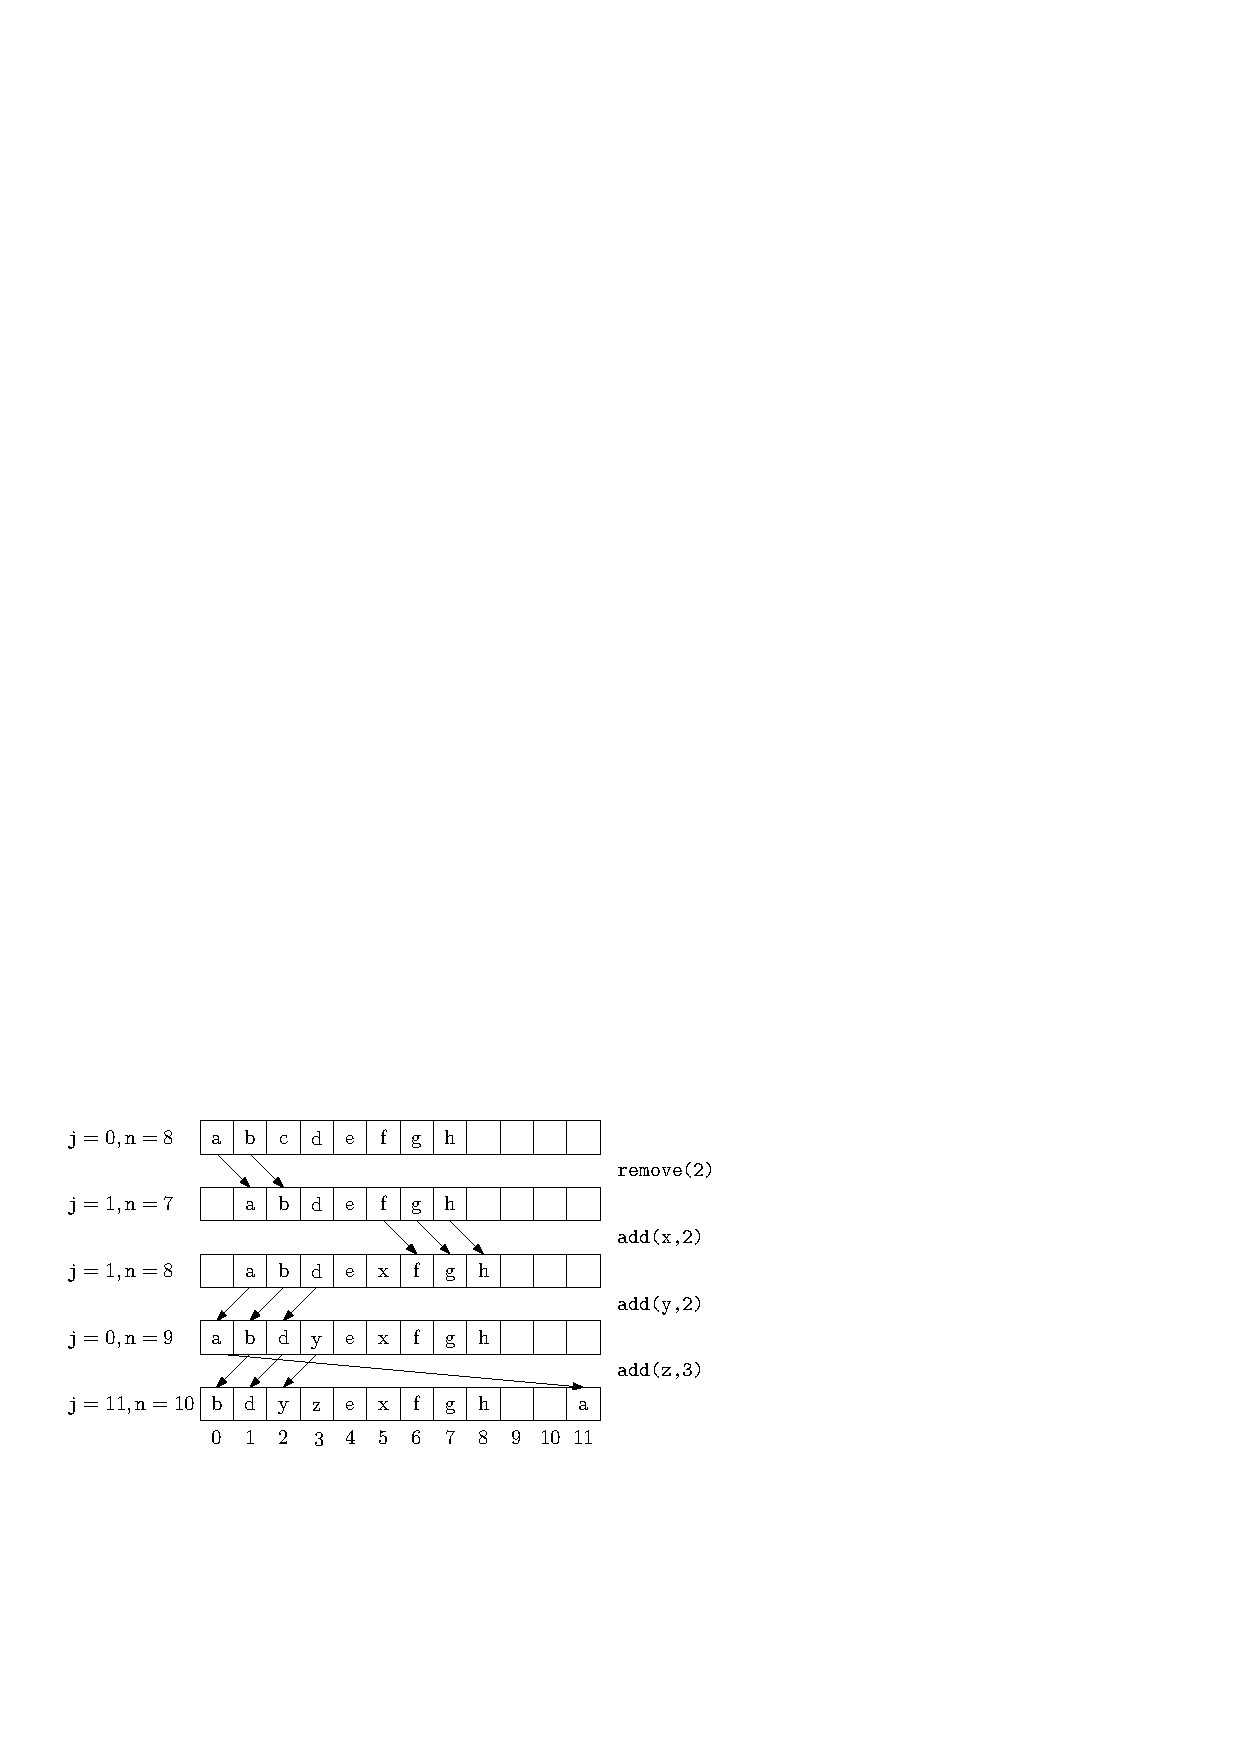
\includegraphics{figs/arraydeque}
  \end{center}
  \caption[Adding and removing from an ArrayDeque]{A sequence of #add(i,x)# and #remove(i)# operations on an
  #ArrayDeque#.  Arrows denote elements being copied.}
  \figlabel{arraydeque}
\end{figure}


\codeimport{ods/ArrayDeque.add(i,x)}

By doing the shifting in this way, we guarantee that #add(i,x)# never
has to shift more than $\min\{ #i#, #n#-#i# \}$ elements.  Thus, the running
time of the #add(i,x)# operation (ignoring the cost of a #resize()#
operation) is $O(1+\min\{#i#,#n#-#i#\})$.

The #remove(i)# operation is similar.  It either shifts elements
$#a[0]#,\ldots,#a[i-1]#$ right by one position or shifts the elements
$#a[i+1]#,\ldots,#a[n-1]#$ left by one position depending on whether
$#i#<#n#/2$.  Again, this means that #remove(i)# never spends more than 
$O(1+\min\{#i#,#n#-#i#\})$ time to shift elements.

\codeimport{ods/ArrayDeque.remove(i)}

\subsection{Summary}

The following theorem summarizes the performance of the #ArrayDeque#
data structure:
\begin{thm}\thmlabel{arraydeque}
  An #ArrayDeque# implements the #List# interface.  Ignoring the cost of
  calls to #resize()#, an #ArrayDeque# supports the operations
  \begin{itemize}
    \item #get(i)# and #set(i,x)# in $O(1)$ time per operation; and
    \item #add(i,x)# and #remove(i)# in $O(1+\min\{#i#,#n#-#i#\})$ time
          per operation.
  \end{itemize}
  Furthermore, beginning with an empty #ArrayDeque#, any sequence of $m$
  #add(i,x)# and #remove(i)# operations results in a total of $O(m)$
  time spent during all calls to #resize()#.
\end{thm}

\section{#DualArrayDeque#: Building a Deque from Two Stacks}
\seclabel{dualarraydeque}

Next, we present another data structure, the #DualArrayDeque# that
achieves the same performance bounds as an #ArrayDeque# by using
two #ArrayStack#s.  Although the asymptotic performance of the
#DualArrayDeque# is no better than that of the #ArrayDeque#, it is
still worth studying since it offers a good example of how to make a
sophisticated data structure by combining two simpler data structures.

A #DualArrayDeque# represents a list using two #ArrayStack#s.  Recall that
an #ArrayStack# is fast when the operations on it modify elements near
the end.  A #DualArrayDeque# places two #ArrayStack#s, called #front#
and #back#, back-to-back so that operations are fast at either end.

\codeimport{ods/DualArrayDeque.front.back}

A #DualArrayDeque# does not explicitly store the number, #n#,
of elements it contains.  It doesn't need to, since it contains
$#n#=#front.size()# + #back.size()#$ elements.  Nevertheless, when
analyzing the #DualArrayDeque# we will still use #n# to denote the number
of elements it contains.

\codeimport{ods/DualArrayDeque.size()}

The #front# #ArrayStack# contains list elements with indices
$0,\ldots,#front.size()#-1$, but stores them in reverse order.
The #back# #ArrayStack# contains list elements with indices
$#front.size()#,\ldots,#size()#-1$ in the normal order.  In this way,
#get(i)# and #set(i,x)# translate into appropriate calls to #get(i)#
or #set(i,x)# on either #front# or #back#, which take $O(1)$ time per operation.

\codeimport{ods/DualArrayDeque.get(i).set(i,x)}

Note that, if an index $#i#<#front.size()#$, then it corresponds to the
element of #front# at position $#front.size()#-#i#-1$, since the
elements of #front# are stored in reverse order.

Adding and removing elements from a #DualArrayDeque# is illustrated in
\figref{dualarraydeque}.  The #add(i,x)# operation manipulates either #front#
or #back#, as appropriate:

\begin{figure}
  \begin{center}
    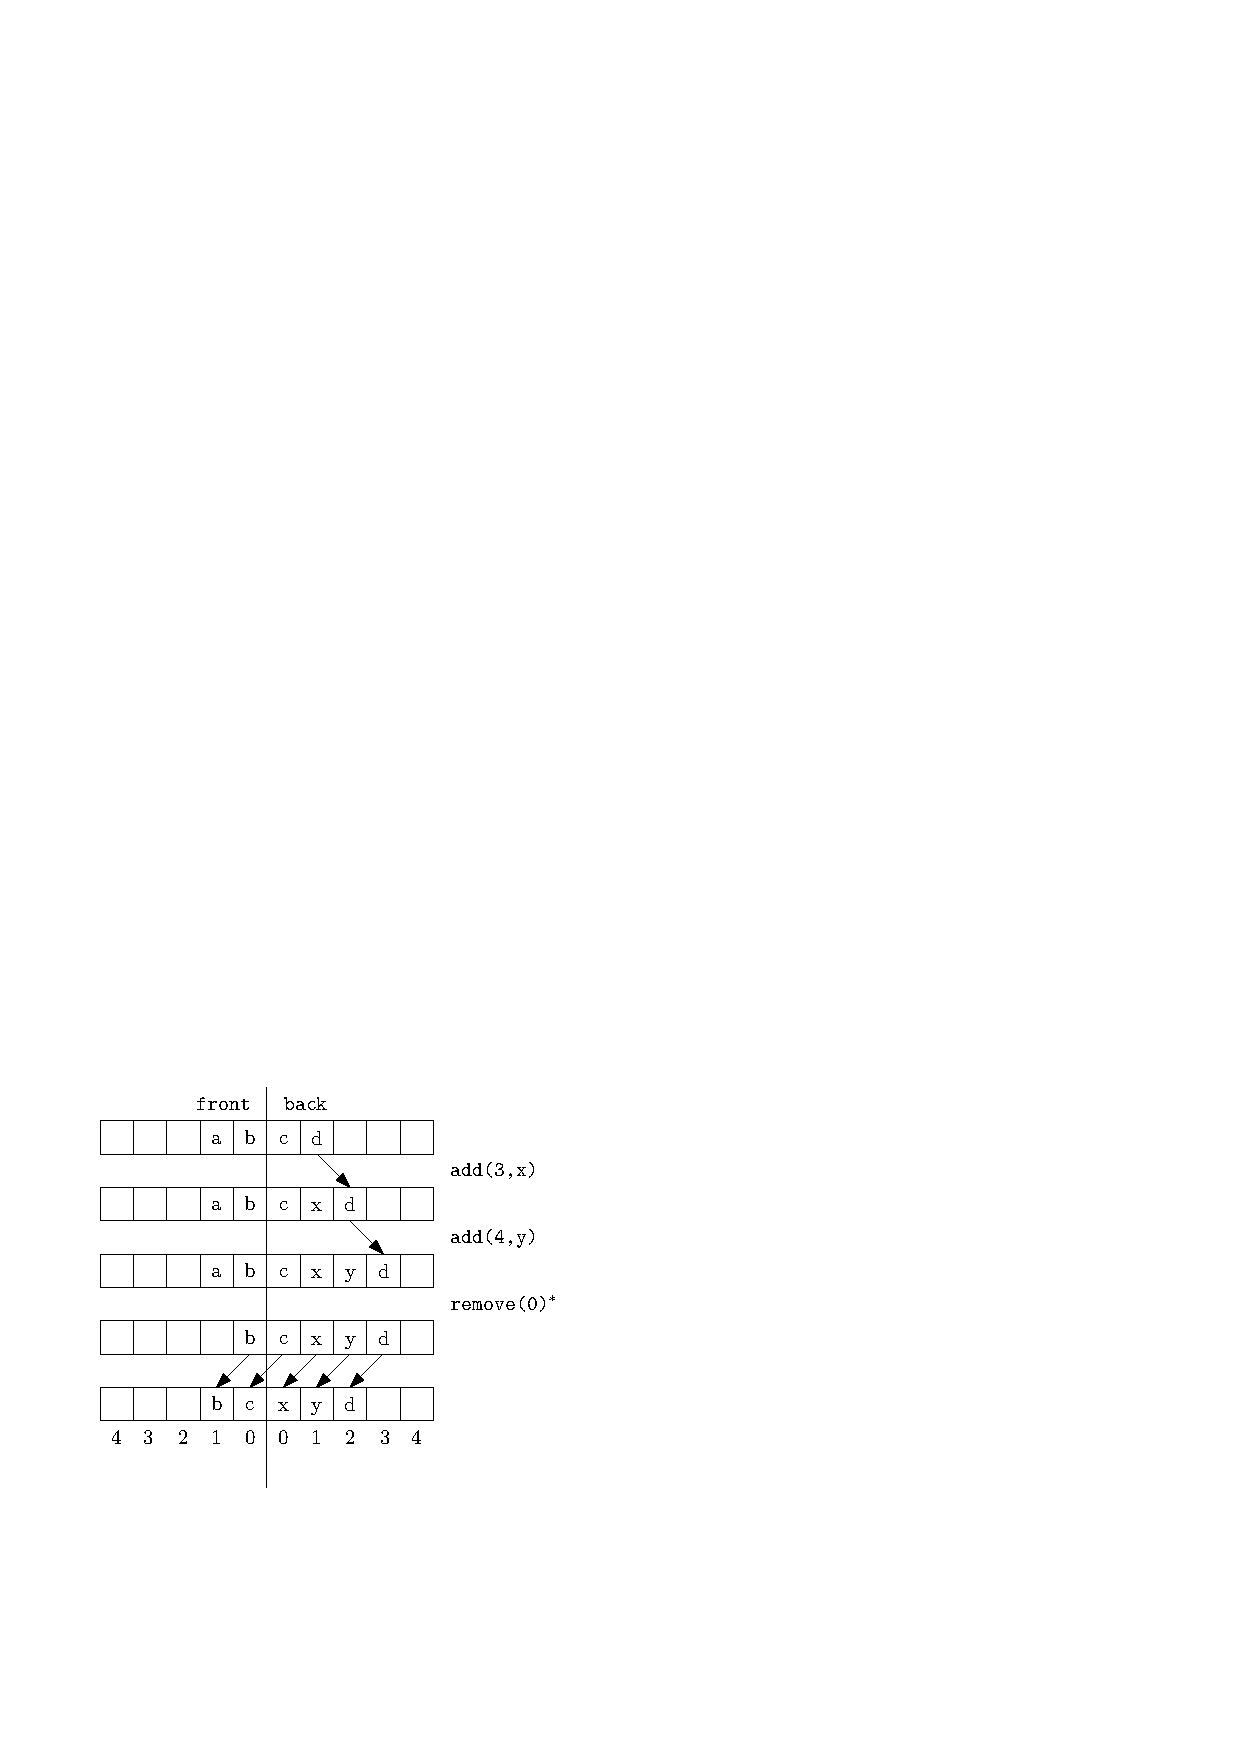
\includegraphics{figs/dualarraydeque}
  \end{center}
  \caption[Adding and removing in a DualArrayDeque]{A sequence of #add(i,x)# and #remove(i)# operations on a
  #DualArrayDeque#.  Arrows denote elements being copied.  Operations that
  result in a rebalancing by #balance()# are marked with an asterisk.}
  \figlabel{dualarraydeque}
\end{figure}



\codeimport{ods/DualArrayDeque.add(i,x)}

The #add(i,x)# method performs rebalancing of the two #ArrayStack#s
#front# and #back#, by calling the #balance()# method.  The
implementation of #balance()# is described below, but for now it is
sufficient to know that #balance()# ensures that, unless $#size()#<2$,
#front.size()# and #back.size()# do not differ by more than a factor
of 3.  In particular, $3\cdot#front.size()# \ge #back.size()#$ and
$3\cdot#back.size()# \ge #front.size()#$.

Next we analyze the cost of #add(i,x)#, ignoring the cost of the
#balance()# operation.  If $#i#<#front.size()#$, then #add(i,x)# becomes 
$#front.add(front.size()-i-1,x)#$.
Since #front# is an #ArrayStack#, the cost of this is 
\begin{equation}
  O(#front.size()#-(#front.size()#-#i#-1)+1) = O(#i#+1) \enspace .
  \eqlabel{das-front}
\end{equation}
On the other hand, if $#i#\ge#front.size()#$, then #add(i,x)# becomes
$#back.add(i-front.size(),x)#$.
The cost of this is 
\begin{equation}
  O(#back.size()#-(#i#-#front.size()#)+1) = O(#n#-#i#+1) \enspace .
  \eqlabel{das-back}
\end{equation}

Notice that the first case \myeqref{das-front} occurs when $#i#<#n#/4$.
The second case \myeqref{das-back} occurs when $#i#\ge 3#n#/4$.  When
$#n#/4\le#i#<3#n#/4$, we can't be sure whether the operation affects
#front# or #back#, but in either case, the operation takes
$O(#n#)=O(#i#)=O(#n#-#i#)$ time, since $#i#\ge #n#/4$ and $#n#-#i#>
#n#/4$.  Summarizing the situation, we have
\[
     \mbox{Running time of } #add(i,x)# \le 
          \left\{\begin{array}{ll}
            O(1+ #i#) & \mbox{if $#i#< #n#/4$} \\
            O(#n#) & \mbox{if $#n#/4 \le #i# < 3#n#/4$} \\
            O(1+#n#-#i#) & \mbox{if $#i# \ge 3#n#/4$}
          \end{array}\right.
\]
Thus, the running time of #add(i,x)# (ignoring the cost of the call to
#balance()#) is $O(1+\min\{#i#, #n#-#i#\})$.

The #remove(i)# operation, and its analysis, is similar to the #add(i,x)#
operation.

\codeimport{ods/DualArrayDeque.remove(i)}

\subsection{Balancing}

Finally, we study the #balance()# operation performed by #add(i,x)#
and #remove(i)#.  This operation is used to ensure that neither #front#
nor #back# gets too big (or too small).  It ensures that, unless there
are fewer than 2 elements, each of #front# and #back# contain at least
$#n#/4$ elements. If this is not the case, then it moves elements between
them so that #front# and #back# contain exactly $\lfloor#n#/2\rfloor$
elements and $\lceil#n#/2\rceil$ elements, respectively.

\codeimport{ods/DualArrayDeque.balance()}

There is not much to analyze.  If the #balance()# operation does
rebalancing, then it moves $\Theta(#n#)$ elements and this takes
$O(#n#)$ time. This is bad, since #balance()# is called with each call to
#add(i,x)# and #remove(i)#.  However, the following lemma shows that, on
average, #balance()# only spends a constant amount of time per operation.

\begin{lem}\lemlabel{dualarraydeque-amortized}
  If an empty #DualArrayDeque# is created and any sequence of $m\ge 1$ calls
  to #add(i,x)# and #remove(i)# are performed, then the total time spent
  during all calls to #balance()# is $O(m)$.
\end{lem}

\begin{proof}
  We will show that, if #balance()# is forced to shift elements,
  then the number of #add(i,x)# and #remove(i)# operations since the
  last time #balance()# shifted any elements is at least $#n#/2-1$.
  As in the proof of \lemref{arraystack-amortized}, this is sufficient
  to prove that the total time spent by #balance()# is $O(m)$.

  We will perform our analysis using the \emph{potential method}.
  Define the \emph{potential} of the #DualArrayDeque# as
  \[  \Phi = |#front.size()# - #back.size()#| \enspace . \]
  The interesting thing about this potential is that a call to #add(i,x)#
  or #remove(i)# that does not do any balancing can increase the potential
  by at most 1.

  Observe that, immediately after a call to #balance()# that shifts
  elements, the potential, $\Phi_0$, is at most 1, since
  \[ \Phi_0 = \left|\lfloor#n#/2\rfloor-\lceil#n#/2\rceil\right|\le 1  \enspace .\]

  Consider the situation immediately before a call to #balance()# that
  shifts elements and suppose, without loss of generality, that #balance()#
  is shifting elements because $3#front.size()# < #back.size()#$.
  Notice that, in this case,
  \begin{eqnarray*}
   #n# & = & #front.size()#+#back.size()# \\
       & < & #back.size()#/3+#back.size()# \\
       & = & \frac{4}{3}#back.size()#
  \end{eqnarray*}
  Furthermore, the potential at this point in time is
  \begin{eqnarray*}
  \Phi_1 & = & #back.size()# - #front.size()# \\
      &>& #back.size()# - #back.size()#/3 \\
      &=& \frac{2}{3}#back.size()# \\
      &>& \frac{2}{3}\times\frac{3}{4}#n# \\
      &=& #n#/2
  \end{eqnarray*}
  Therefore, the number of calls to #add(i,x)# or #remove(i)# since
  the last time #balance()# shifted elements is at least $\Phi_1-\Phi_0
  > #n#/2-1$. This completes the proof.
\end{proof}

\subsection{Summary}

The following theorem summarizes the performance of a #DualArrayStack#

\begin{thm}\thmlabel{dualarraydeque}
  A #DualArrayDeque# implements the #List# interface.  Ignoring the
  cost of calls to #resize()# and #balance()#, a #DualArrayDeque#
  supports the operations
  \begin{itemize}
    \item #get(i)# and #set(i,x)# in $O(1)$ time per operation; and
    \item #add(i,x)# and #remove(i)# in $O(1+\min\{#i#,#n#-#i#\})$ time
          per operation.
  \end{itemize}
  Furthermore, beginning with an empty #DualArrayDeque#, any sequence of $m$
  #add(i,x)# and #remove(i)# operations results in a total of $O(m)$
  time spent during all calls to #resize()# and #balance()#.
\end{thm}


\section{#RootishArrayStack#: A Space-Efficient Array Stack}
\seclabel{rootisharraystack}

One of the drawbacks of all previous data structures in this chapter
is that, because they store their data in one or two arrays, and they
avoid resizing these arrays too often, the arrays are frequently not
very full.  For example, immediately after a #resize()# operation on
an #ArrayStack#, the backing array #a# is only half full.  Even worse,
there are times when only $1/3$ of #a# contains data.

In this section, we discuss a data structure, the #RootishArrayStack#,
that addresses the problem of wasted space.  The #RootishArrayStack#
stores #n# elements using $O(\sqrt{#n#})$ arrays.  In these arrays, at
most $O(\sqrt{#n#})$ array locations are unused at any time.  All
remaining array locations are used to store data.  Therefore, these
data structures waste at most $O(\sqrt{#n#})$ space when storing #n#
elements.

A #RootishArrayStack# stores its elements in a list of #r#
arrays called \emph{blocks} that are numbered $0,1,\ldots,#r#-1$.
See \figref{rootisharraystack}.  Block $b$ contains $b+1$ elements.
Therefore, all #r# blocks contain a total of
\[
  1+ 2+ 3+\cdots +#r# = #r#(#r#+1)/2
\]
elements.  The above formula (allegedly discovered by the
mathematician Gau\ss\ at the age of 9) can be obtained as shown in
\figref{gauss}.

\begin{figure}
  \begin{center}
    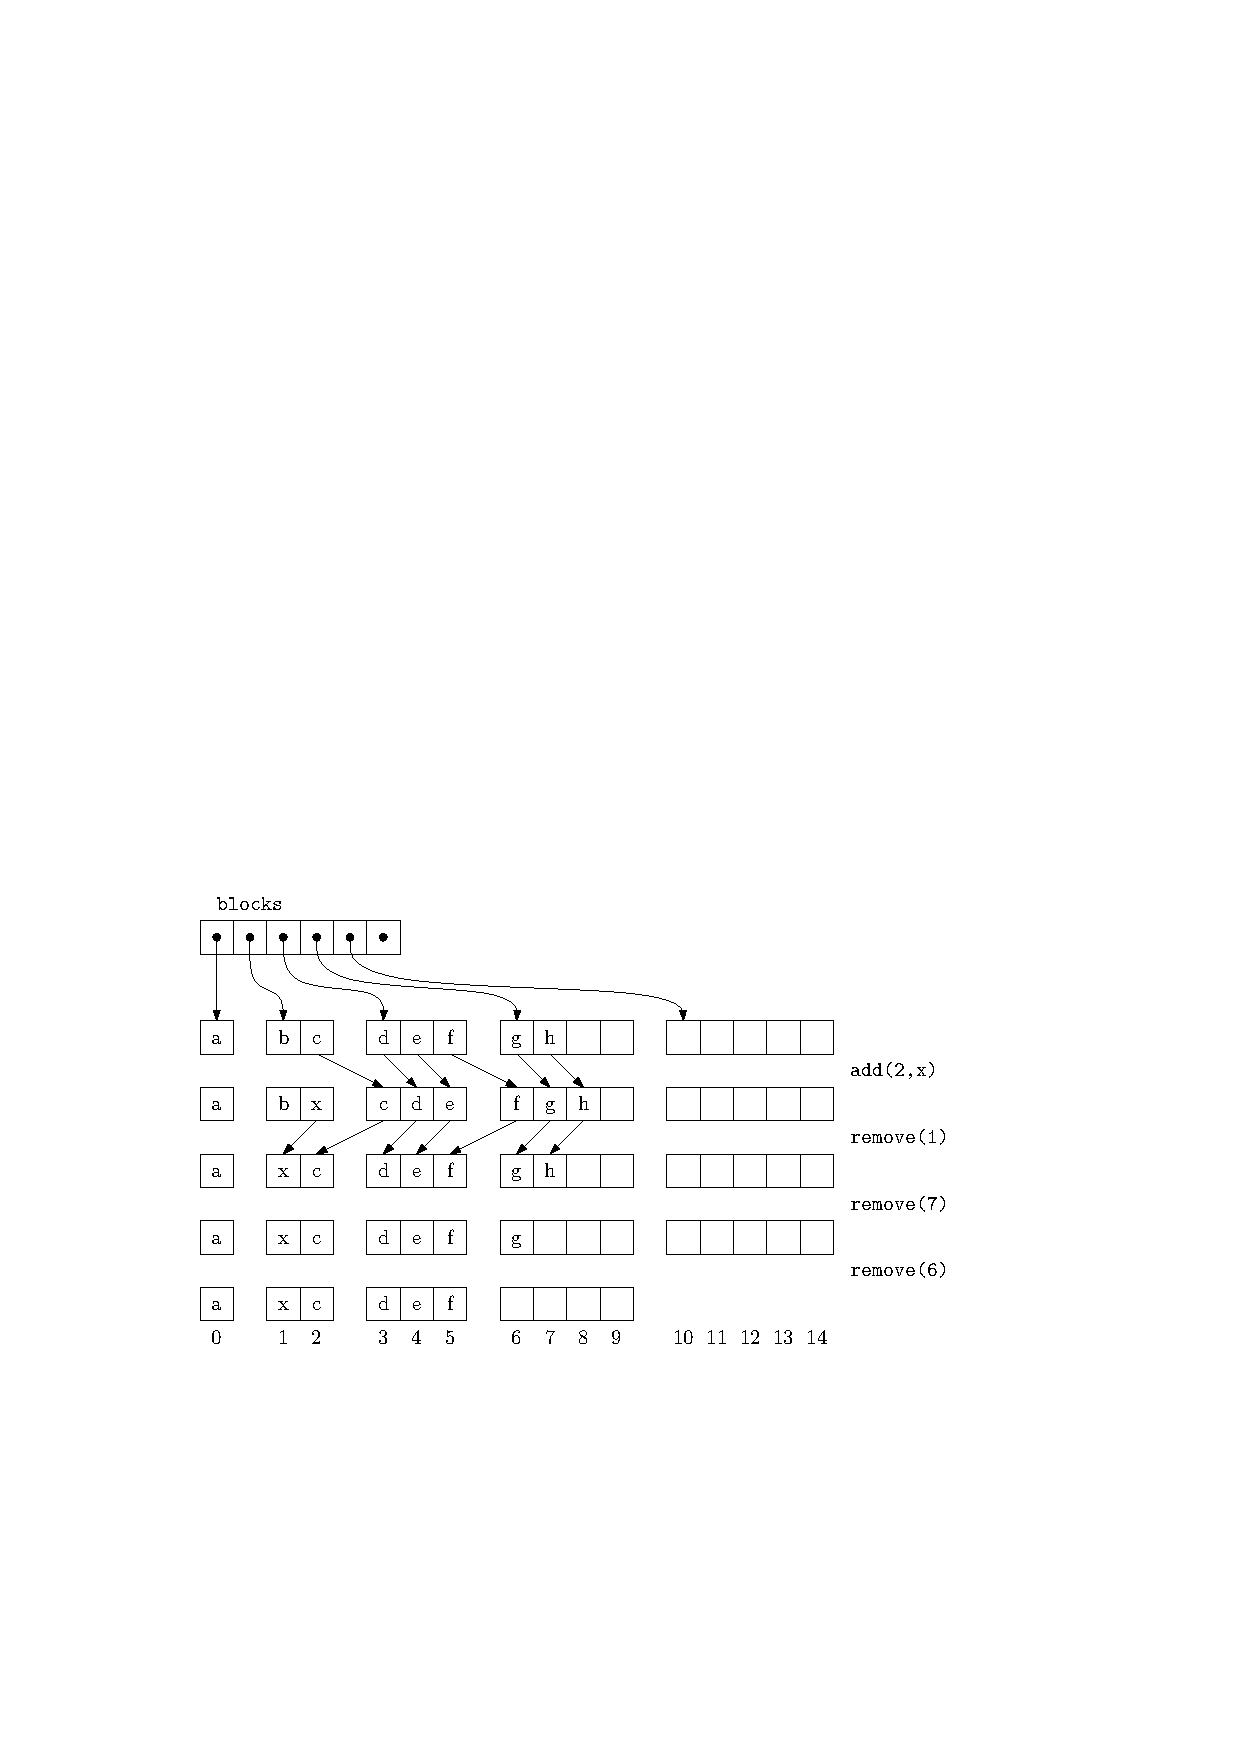
\includegraphics{figs/rootisharraystack}
  \end{center}
  \caption[Adding and removing in a RootishArrayStack]{A sequence of #add(i,x)# and #remove(i)# operations on a
  #RootishArrayStack#.  Arrows denote elements being copied. }
  \figlabel{rootisharraystack}
\end{figure}

\codeimport{ods/RootishArrayStack.blocks.n}

\begin{figure}
  \begin{center}
    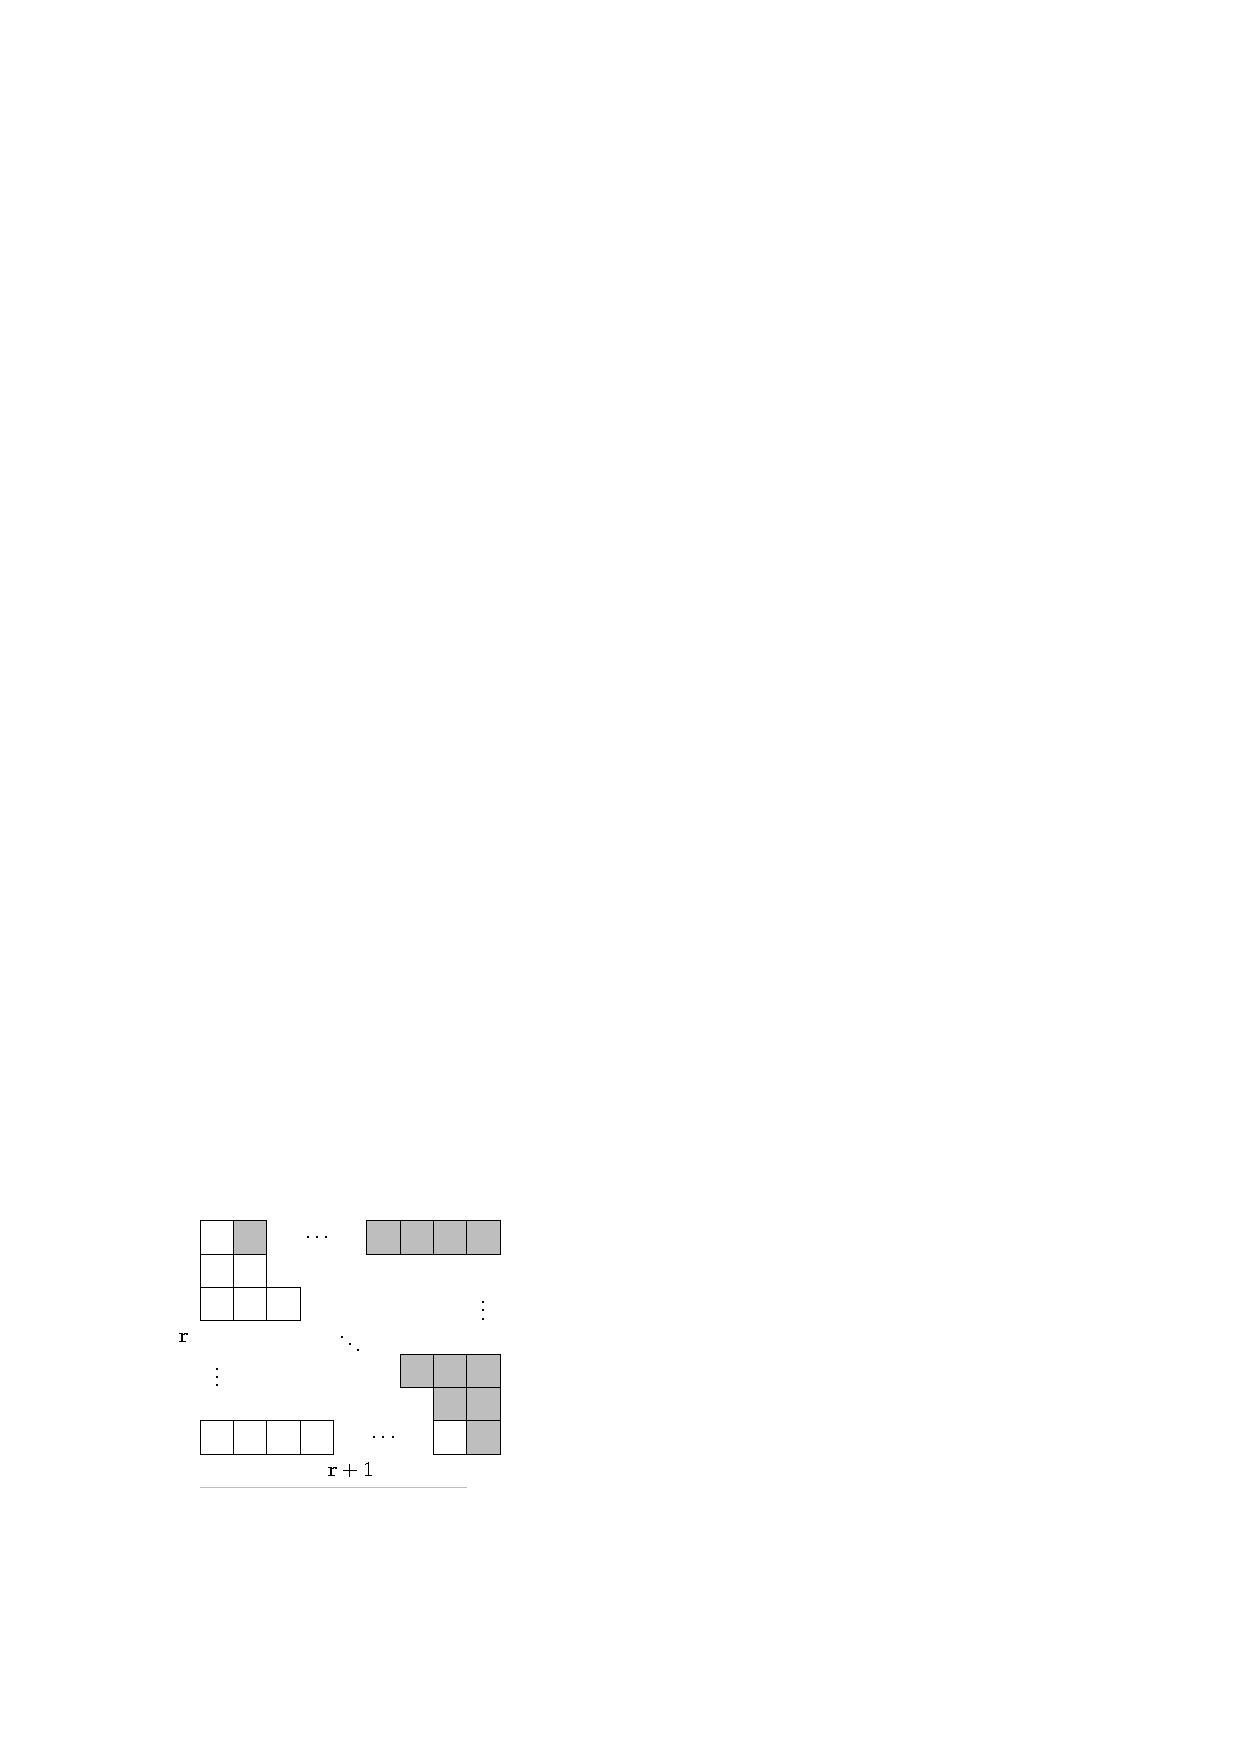
\includegraphics{figs/gauss}
  \end{center}
  \caption{The number of white squares is $1+2+3+\cdots+#r#$.  The number of
  shaded squares is the same.  Together the white and shaded squares make a
  rectangle consisting of $#r#(#r#+1)$ squares.}
  \figlabel{gauss}
\end{figure}

The elements of the list are laid out in the blocks as we might
expect.  The list element with index 0 is stored in block 0, the
elements with list indices 1 and 2 are stored in block 1, the elements
with list indices 3, 4, and 5 are stored in block 2, and so on.  The
main problem we have to address is that of determining, given an index
$#i#$, which block contains #i# as well as the index corresponding to
#i# within that block.

Determining the index of #i# within its block turns out to be easy. If
index #i# is in block #b#, then the number of elements in blocks
$0,\ldots,#b#-1$ is $#b#(#b#+1)/2$.  Therefore, #i# is stored at location
\[
     #j# = #i# - #b#(#b#+1)/2
\]
within block #b#.  Somewhat more challenging is the problem of determining
the value of #b#.  The number of elements that have indices less than
or equal to #i# is $#i#+1$.  On the other hand, the number of elements
in blocks 0,\ldots,b is $(#b#+1)(#b#+2)/2$.  Therefore, #b# is the smallest
integer such that
\[
    (#b#+1)(#b#+2)/2 \ge #i#+1 \enspace .
\]
We can rewrite this equation as
\[
    #b#^2 + 3#b# - 2#i# \ge  0 \enspace .
\]
The corresponding quadratic equation $#b#^2 + 3#b# - 2#i# =  0$ has two
solutions: $#b#=(-3 + \sqrt{9+8#i#}) / 2$ and $#b#=(-3 - \sqrt{9+8#i#}) / 2$.
The second solution makes no sense in our application since it always
gives a negative value. Therefore, we obtain the solution $#b# = (-3 +
\sqrt{9+8i}) / 2$.  In general, this solution is not an integer, but
going back to our inequality, we want the smallest integer $#b#$ such that 
$#b# \ge (-3 + \sqrt{9+8i}) / 2$.  This is simply
\[
   #b# = \left\lceil(-3 + \sqrt{9+8i}) / 2\right\rceil \enspace .
\]

\codeimport{ods/RootishArrayStack.i2b(i)}

With this out of the way, the #get(i)# and #set(i,x)# methods are straightforward.  We first compute the appropriate block #b# and the appropriate index #j# within the block and then perform the appropriate operation:

\codeimport{ods/RootishArrayStack.get(i).set(i,x)}

If we use any of the data structures in this chapter for representing the #blocks# list, then #get(i)# and #set(i,x)# will each run in constant time.

The #add(i,x)# method will, by now, look familiar.  We first check if
our data structure is full, by checking if the number of blocks #r#
is such that $#r#(#r#+1)/2 = #n#$ and, if so, we call #grow()#
to add another block.  With this done, we shift elements with indices
$#i#,\ldots,#n#-1$ to the right by one position to make room for the
new element with index #i#:

\codeimport{ods/RootishArrayStack.add(i,x)}

The #grow()# method does what we expect. It adds a new block:

\codeimport{ods/RootishArrayStack.grow()}

Ignoring the cost of the #grow()# operation, the cost of an #add(i,x)#
operation is dominated by the cost of shifting and is therefore
$O(1+#n#-#i#)$, just like an #ArrayStack#.

The #remove(i)# operation is similar to #add(i,x)#.  It shifts the
elements with indices $#i#+1,\ldots,#n#$ left by one position and then,
if there is more than one empty block, it calls the #shrink()# method
to remove all but one of the unused blocks:

\codeimport{ods/RootishArrayStack.remove(i)}
\codeimport{ods/RootishArrayStack.shrink()}

Once again, ignoring the cost of the #shrink()# operation, the cost of
a #remove(i)# operation is dominated by the cost of shifting  and is
therefore $O(#n#-#i#)$.

\subsection{Analysis of Growing and Shrinking}

The above analysis of #add(i,x)# and #remove(i)# does not account for
the cost of #grow()# and #shrink()#.  Note that, unlike the
#ArrayStack.resize()# operation, #grow()# and #shrink()# do not do any
copying of data.  They only allocate or free an array of size #r#.  In
some environments, this takes only constant time, while in others, it
may require $\Theta(#r#))$ time.

We note that, immediately after a call to #grow()# or #shrink()#, the
situation is clear. The final block is completely empty and all other
blocks are completely full.  Another call to #grow()# or #shrink()# will
not happen until at least $#r#-1$ elements have been added or removed.
Therefore, even if #grow()# and #shrink()# take $O(#r#)$ time, this
cost can be amortized over at least $#r#-1$ #add(i,x)# or #remove(i)#
operations, so that the amortized cost of #grow()# and #shrink()# is
$O(1)$ per operation.

\subsection{Space Usage}
\seclabel{rootishspaceusage}

Next, we analyze the amount of extra space used by a #RootishArrayStack#.
In particular, we want to count any space used by a #RootishArrayStack# that is not an array element currently used to hold a list element.  We call all such space \emph{wasted space}.

The #remove(i)# operation ensures that a #RootishArrayStack# never has
more than 2 blocks that are not completely full.  The number of blocks,
#r#, used by a #RootishArrayStack# that stores #n# elements therefore
satisfies
\[
    (#r#-2)(#r#-1) \le #n#
\]
Again, using the quadratic equation on this gives
\[
   #r# \le (3+\sqrt{1+4#n#})/2 = O(\sqrt{#n#})
\]
The last two blocks have sizes #r# and #r-1#, so the space wasted by these
two blocks is at most $2#r#-1 = O(\sqrt{#n#})$.  If we store the blocks
in (for example) an #ArrayList#, then the amount of space wasted by the
#List# that stores those #r# blocks is also $O(#r#)=O(\sqrt{#n#})$.  The
other space needed for storing #n# and other accounting information is $O(1)$.
Therefore, the total amount of wasted space in a #RootishArrayStack#
is $O(\sqrt{#n#})$.

Next, we argue that this space usage is optimal for any data structure
that starts out empty and can support the addition of one item at a
time. More precisely, we will show that, at some point during the
addition of #n# items, the data structure is wasting an amount of
space at least in $\sqrt{#n#}$ (though it may be only wasted for a
moment).

Suppose we start with an empty data structure and we add #n# items
one at a time.  At the end of this process, all #n# items are stored
in the structure and they are distributed among a collection of #r#
memory blocks.  If $#r#\ge \sqrt{#n#}$, then the data structure must be
using #r# pointers (or references) to keep track of these #r# blocks,
and this is wasted space.  On the other hand, if $#r# < \sqrt{#n#}$
then, by the pigeonhole principle, some block must have size at least
$#n#/#r# > \sqrt{#n#}$.  Consider the moment at which this block was
first allocated.  Immediately after it was allocated, this block was
empty, and was therefore wasting $\sqrt{#n#}$ space.  Therefore, at some
point in time during the insertion of #n# elements, the data structure was
wasting $\sqrt{#n#}$ space.

\subsection{Summary}

The following theorem summarizes the performance of the #RootishArrayStack#
data structure:

\begin{thm}\thmlabel{rootisharraystack}
  A #RootishArrayStack# implements the #List# interface.  Ignoring the cost of
  calls to #grow()# and #shrink()#, a #RootishArrayStack# supports the operations
  \begin{itemize}
    \item #get(i)# and #set(i,x)# in $O(1)$ time per operation; and
    \item #add(i,x)# and #remove(i)# in $O(1+#n#-#i#)$ time per operation.
  \end{itemize}
  Furthermore, beginning with an empty #RootishArrayStack#, any sequence of $m$
  #add(i,x)# and #remove(i)# operations results in a total of $O(m)$
  time spent during all calls to #grow()# and #shrink()#.

  The space (measured in words)\footnote{Recall \secref{model} for a
  discussion of how memory is measured.} used by a #RootishArrayStack#
  that stores #n# elements is $#n# +O(\sqrt{#n#})$.
\end{thm}

\subsection{Computing Square Roots}

A reader who has had some exposure to models of computation may notice
that the #RootishArrayStack#, as described above, does not fit into
the usual word-RAM model of computation (\secref{model}) because it
requires taking square roots.  The square root operation is generally
not considered a basic operation and is therefore not usually part of
the word-RAM model.

In this section, we take time to show that the square root operation can
be implemented efficiently.  In particular, we show that for any integer
$#x#\in\{0,\ldots,#n#\}$,  $\lfloor\sqrt{#x#}\rfloor$ can be computed
in constant-time, after $O(\sqrt{#n#})$ preprocessing that creates two
arrays of length $O(\sqrt{#n#})$. 
The following lemma shows that we can reduce the problem of computing the square root of #x# to the square root of a related value #x'#.

\begin{lem}\lemlabel{root}
Let $#x#\ge 1$ and let $#x'#=#x#-a$, where $0\le a\le\sqrt{#x#}$.  Then
   $\sqrt{x'} \ge \sqrt{#x#}-1$.
\end{lem}

\begin{proof}
It suffices to show that
\[
\sqrt{#x#-\sqrt{#x#}} \ge \sqrt{#x#}-1 \enspace .
\]
Square both sides of this inequality to get
\[
 #x#-\sqrt{#x#} \ge #x#-2\sqrt{#x#}+1
\]
and gather terms to get 
\[
 \sqrt{#x#} \ge 1
\]
which is clearly true for any $#x#\ge 1$.
\end{proof}

Start by restricting the problem a little, and assume that $2^{#r#} \le
#x# < 2^{#r#+1}$, so that $\lfloor\log #x#\rfloor=#r#$, i.e., #x# is an
integer having $#r#+1$ bits in its binary representation.  We can take
$#x'#=#x# - (#x#\bmod 2^{\lfloor r/2\rfloor})$.  Now, #x'# satisfies
the conditions of \lemref{root}, so $\sqrt{#x#}-\sqrt{#x'#} \le 1$.
Furthermore, #x'# has all of its lower-order $\lfloor #r#/2\rfloor$ bits
equal to 0, so there are only
\[
  2^{#r#+1-\lfloor #r#/2\rfloor} \le 4\cdot2^{#r#/2} \le 4\sqrt{#x#}
\]
possible values of #x'#.  This means that we can use an array, #sqrttab#,
that stores the value of $\lfloor\sqrt{#x'#}\rfloor$ for each possible
value of #x'#.  A little more precisely, we have
\[
   #sqrttab#[i] 
    = \left\lfloor
       \sqrt{i 2^{\lfloor #r#/2\rfloor}}
      \right\rfloor \enspace .
\]
In this way, $#sqrttab#[i]$ is within 2 of $\sqrt{#x#}$ for all
$#x#\in\{i2^{\lfloor r/2\rfloor},\ldots,(i+1)2^{\lfloor r/2\rfloor}-1\}$.
Stated another way, the array entry 
$#s#=#sqrttab#[#x##>>#\lfloor #r#/2\rfloor]$ is either equal to
$\lfloor\sqrt{#x#}\rfloor$,
$\lfloor\sqrt{#x#}\rfloor-1$, or
$\lfloor\sqrt{#x#}\rfloor-2$.  From #s# we can determine the value
of $\lfloor\sqrt{#x#}\rfloor$ by
incrementing #s# until 
$(#s#+1)^2 > #x#$.
\codeimport{ods/FastSqrt.sqrt(x,r)}

Now, this only works for $#x#\in\{2^{#r#},\ldots,2^{#r#+1}-1\}$ and
#sqrttab# is a special table that only works for a particular value
of $#r#=\lfloor\log #x#\rfloor$.  To overcome this, we could compute
$\lfloor\log #n#\rfloor$ different #sqrttab# arrays, one for each possible
value of $\lfloor\log #x#\rfloor$. The sizes of these tables form an exponential sequence whose largest value is at most $4\sqrt{#n#}$, so the total size of all tables is $O(\sqrt{#n#})$.

However, it turns out that more than one #sqrttab# array is unnecessary;
we only need one #sqrttab# array for the value $#r#=\lfloor\log
#n#\rfloor$.  Any value #x# with $\log#x#=#r'#<#r#$ can be \emph{upgraded}
by multiplying #x# by $2^{#r#-#r'#}$ and using the equation
\[
    \sqrt{2^{#r#-#r'#}x} = 2^{(#r#-#r#')/2}\sqrt{#x#} \enspace .
\]
The quantity $2^{#r#-#r#'}x$ is in the range
$\{2^{#r#},\ldots,2^{#r#+1}-1\}$ so we can look up its square root
in #sqrttab#.  The following code implements this idea to compute
$\lfloor\sqrt{#x#}\rfloor$ for all non-negative integers #x# in the
range $\{0,\ldots,2^{30}-1\}$ using an array, #sqrttab#, of size $2^{16}$.
\codeimport{ods/FastSqrt.sqrt(x)}

Something we have taken for granted thus far is the question of how
to compute
$#r#'=\lfloor\log#x#\rfloor$.  Again, this is a problem that can be solved
with an array, #logtab#, of size $2^{#r#/2}$.  In this case, the
code is particularly simple, since $\lfloor\log #x#\rfloor$ is just the
index of the most significant 1 bit in the binary representation of #x#.
This means that, for $#x#>2^{#r#/2}$, we can right-shift the bits of
#x# by $#r#/2$ positions before using it as an index into #logtab#.
The following code does this using an array #logtab# of size $2^{16}$ to compute
$\lfloor\log #x#\rfloor$ for all #x# in the range $\{1,\ldots,2^{32}-1\}$
\codeimport{ods/FastSqrt.log(x)}

Finally, for completeness, we include the following code that initializes #logtab# and #sqrttab#:
\codeimport{ods/FastSqrt.inittabs()}

To summarize, the computations done by the #i2b(i)# method can be
implemented in constant time on the word-RAM using $O(\sqrt{n})$ extra
memory to store the #sqrttab# and #logtab# arrays.  These arrays can be
rebuilt when #n# increases or decreases by a factor of 2, and the cost
of this rebuilding can be amortized over the number of #add(i,x)# and
#remove(i)# operations that caused the change in #n# in the same way that
the cost of #resize()# is analyzed in the #ArrayStack# implementation.


\section{Discussion and Exercises}

Most of the data structures described in this chapter are folklore. They
can be found in implementations dating back over 30 years.  For example,
implementations of stacks, queues, and deques which generalize easily
to the #ArrayStack#, #ArrayQueue# and #ArrayDeque# structures described
here are discussed by Knuth \cite[Section~2.2.2]{k97v1}.

Brodnik \etal\ \cite{bcdms99} seem to have been the first to describe
the #RootishArrayStack# and prove a $\sqrt{n}$ lower-bound like that
in \secref{rootishspaceusage}.  They also present a different structure
that uses a more sophisticated choice of block sizes in order to avoid
computing square roots in the #i2b(i)# method.  With their scheme, the
block containing #i# is block $\lfloor\log (#i#+1)\rfloor$, which is just
the index of the leading 1 bit in the binary representation of $#i#+1$.
Some computer architectures provide an instruction for computing the
index of the leading 1-bit in an integer.

A structure related to the #RootishArrayStack# is the $2$-level
\emph{tiered-vector} of Goodrich and Kloss \cite{gk99}.  This structure
supports #get(i,x)# and #set(i,x)# in constant time and #add(i,x)# and
#remove(i)# in $O(\sqrt{#n#})$ time.  These running times are similar
to what can be achieved with the more careful implementation of a
#RootishArrayStack# discussed in \excref{rootisharraystack-fast}.

%\javaonly{
%\begin{exc}
%  In the #ArrayStack# implementation, after the first call to #remove(i)#,
%  the backing array, #a#, contains #n# non-#null# values even though
%  the #ArrayStack# only contains #n# elements.  Where is the extra
%  non-#null# value.  Discuss any consequences this has on the Java Runtime Environment's memory manager.
%\end{exc}
%}

\begin{exc}
  The #List# method #addAll(i,c)# inserts all elements of the #Collection#
  #c# into the list at position #i#.  (The #add(i,x)# method is a special
  case where $#c#=\{#x#\}$.)  Explain why, for the data structures
  in this chapter, it is not efficient to implement #addAll(i,c)# by
  repeated calls to #add(i,x)#.  Design and implement a more efficient
  implementation.
\end{exc}

\begin{exc}
  Design and implement a #RandomQueue#.  This is an implementation
  of the #Queue# interface in which the #remove()# operation removes an
  element that is chosen uniformly at random among all the elements in
  the queue.  The #add(x)# and #remove()# operations in a #RandomQueue#
  should take constant time.
\end{exc}

\begin{exc}
  Design and implement a #Treque# (triple-ended queue). This is a #List#
  implementation in which #get(i)# and #set(i,x)# run in constant time
  and #add(i,x)# and #remove(i)# run in time
  \[
     O(1+\min\{#i#, #n#-#i#, |#n#/2-#i#|\}) \enspace .
  \]
  With this running time, modifications are fast if they are near either
  end or near the middle of the list.
\end{exc}

\begin{exc}
  Implement a method #rotate(r)# that ``rotates'' a #List# so that
  list item #i# becomes list item $(#i#+#r#)\bmod n$.  When run on
  an #ArrayDeque#, or a #DualArrayDeque#, #rotate(r)# should run in
  $O(1+\min\{r,n-r\})$.
\end{exc}

\begin{exc}
  Modify the #ArrayDeque# implementation so that the shifting
  done by #add(i,x)#, #remove(i)#, and #resize()# is done using
  #System.arraycopy(s,i,d,j,n)#.
\end{exc}

\begin{exc}
  Modify the #ArrayDeque# implementation so that it does not use the
  #%# operator (which is expensive on some systems).  Instead, it
  should make use of the fact that, if #a.length# is a power of 2,
  then #k%a.length#$=$#k&(a.length-1)#. (Here, #&# is the bitwise-and
  operator.)
\end{exc}

\begin{exc}
  Design and implement a variant of #ArrayDeque# that does not do any
  modular arithmetic at all.  Instead, all the data sits in a consecutive
  block, in order, inside an array.  When the data overruns the beginning
  or the end of this array, a modified #rebuild()# operation is performed.
  The amortized cost of all operations should be the same as in an
  #ArrayDeque#.

  Hint: Making this work is really all about how a #rebuild()# operation
  is performed.  You would like #rebuild()# to put the data structure
  into a state where the data cannot run off either end until at least
  $#n#/2$ operations have been performed.

  Test the performance of your implementation against the #ArrayDeque#.
  Optimize your implementation (by using #System.arraycopy(a,i,b,i,n)#)
  and see if you can get it to outperform the #ArrayDeque# implementation.
\end{exc}

\begin{exc}
  Design and implement a version of a #RootishArrayStack# that has
  only $O(\sqrt{#n#})$ wasted space, but that can perform #add(i,x)#
  and #remove(i,x)# operations in $O(1+\min\{#i#,#n#-#i#\})$ time.
\end{exc}

\begin{exc}\exclabel{rootisharraystack-fast}
  Design and implement a version of a #RootishArrayStack# that has
  only $O(\sqrt{#n#})$ wasted space, but that can perform #add(i,x)#
  and #remove(i,x)# operations in $O(1+\min\{\sqrt{#n#},#n#-#i#\})$
  time. (For an idea on how to do this, see \secref{selist}.)
\end{exc}

\begin{exc}
  Design and implement a version of a #RootishArrayStack# that has
  only $O(\sqrt{#n#})$ wasted space, but that can perform #add(i,x)# and
  #remove(i,x)# operations in $O(1+\min\{#i#,\sqrt {#n#},#n#-#i#\})$ time.
  (See \secref{selist} for ideas on how to achieve this.)
\end{exc}


